\documentclass[xcolor=dvipsnames]{beamer} 
\usepackage{natbib}                 % fancy bibliography.
\usepackage{url}                    % allow printing of urls.
\usepackage{dsfont}
\usepackage{amsmath}
\usepackage{wrapfig}
\usepackage{epstopdf}
\usepackage{listings}

\usepackage{color}

\usepackage{caption}
\setbeamertemplate{footline}[frame number]
\captionsetup{font=scriptsize,labelfont=bf}


\title{\textbf{An introduction to Python}}

\date{}


\definecolor{dkgreen}{rgb}{0,0.6,0}
\definecolor{gray}{rgb}{0.5,0.5,0.5}
\definecolor{mauve}{rgb}{0.58,0,0.82}

\lstset{frame=tb,
  language=Python,
  aboveskip=3mm,
  belowskip=3mm,
  showstringspaces=false,
  columns=flexible,
  basicstyle={\small},
  numbers=none,
  numberstyle=\tiny\color{gray},
  keywordstyle=\color{blue},
  commentstyle=\color{dkgreen},
  stringstyle=\color{mauve},
  breaklines=true,
  breakatwhitespace=true
  tabsize=3
}

\begin{document}
\lstset{language=Python}

\begin{frame}[t]
  \maketitle
  \vskip -9em
\end{frame}

\AtBeginSection[] % Do nothing for \section*
{ 
  \frame<beamer>
    {
          \frametitle{Contents}
	        \tableofcontents[current]
	}
}



\section{Why Python?}

\begin{frame}
\frametitle{Our needs}

\begin{itemize}
\item Get data (simulation, experiment control)
\item Manipulate and process data.
\item Visualize results... to understand what we are doing!
\end{itemize}

\end{frame}


\begin{frame}
\frametitle{What is programming?}

\begin{figure}
\begin{center}

\includegraphics{images/bricks.jpg}
\end{center}
\end{figure}
\end{frame}


\begin{frame}
\frametitle{Why Python?}
\begin{itemize}
\item Readable and well structured language
\item Quick development and execution time
\item Rich collections of existing bricks
\end{itemize}
\end{frame}

\begin{frame}
\frametitle{Setting up Python}
\textit{(For windows)}
\begin{itemize}
\item Download from the official website
\item Use a "all in one" package installer: Anaconda, canopy...
\end{itemize}

\vspace{2em}
To test if python is installed correctly, type \texttt{python} in a terminal.
\end{frame}

\section{The basics}

\begin{frame}
\begin{block}{Value or object}
\frametitle{Values and Data Types}
A \textbf{value} (or an \textbf{object}) is one of the fundamental thing that
a program manipulates. Objects are classified into different \textbf{types} or
\textbf{class}.
\end{block}

\vspace{1em}
\lstinputlisting[language=Python]{src/values.py}
\end{frame}

\begin{frame}
\frametitle{Data Types}

\begin{tabular}{l | l}
boolean & \texttt{True}, \texttt{False} \\
string & \texttt{'Hello world'}, \texttt{"I'm a computer scientist"} \\
integer & \texttt{5} \\
float & \texttt{1.} \\ 
complex & \texttt{1 + 1j}
\end{tabular}

\vspace{1em}
\begin{alertblock}{Question}
\begin{itemize}
\item What is the type of the following values: "3", '5' ?
\end{itemize}
\end{alertblock}
\end{frame}

\begin{frame}
\frametitle{Using Python as a calculator}

The \textbf{interpreter} can be used as a simple calculator.

\vspace{1em}
\lstinputlisting[language=Python]{src/calculator.py}

\vspace{1em}
\begin{alertblock}{Question}
\begin{itemize}
\item Do you understand all the outputs?
\item What do you think the pound (\texttt{\#}) sign means?
\end{itemize}
\end{alertblock}
\end{frame}


\begin{frame}
\frametitle{Using Python to compare}

Several operators (\texttt{>}, \texttt{==}, \texttt{!=}, \texttt{<=}) can be
used to compared values of same or different types.

\vspace{1em}
\lstinputlisting[language=Python]{src/comparison.py}
\end{frame}

\begin{frame}
\frametitle{Variables and assignments}
\begin{block}{Variables}

A \textbf{variable} is a name that refers to a value.
A value is \textbf{assigned} to a variable.
\end{block}
\vspace{1em}
\lstinputlisting[language=Python]{src/variables.py}

\vspace{1em}
\begin{alertblock}{Question}
\begin{itemize}
\item What are the types of \texttt{a} and \texttt{b}?
\item What is the type of \texttt{c}?
\end{itemize}
\end{alertblock}
\end{frame}

\begin{frame}
\frametitle{Variables and assigments}
\begin{itemize}
\item A variable is just a name.
\item You must assign a value to a variable before using it.
\end{itemize}
\lstinputlisting{src/variables_1.py}
\end{frame}

\begin{frame}
\frametitle{A few Python built-in functions}

\begin{block}{Function}
A \textbf{function} is a block of code that takes in input no, one or many \textbf{arguments}
and returns something (often a value).
\end{block}

\begin{minipage}[tl]{0.45\textwidth}
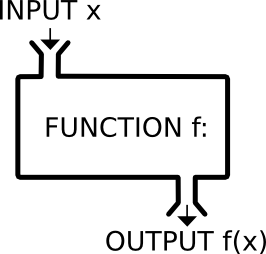
\includegraphics[width=60px]{images/Function_machine2.png}
\end{minipage}

\begin{minipage}[tr]{0.45\textwidth}
\lstinputlisting{src/_builtins.py}
\end{minipage}
\end{frame}

\begin{frame}
\frametitle{A few Python built-ins}
\scriptsize
\begin{tabular}{lllll}
\texttt{abs()} & \texttt{divmod()} & \texttt{input()} & \texttt{open()} & \texttt{staticmethod()} \\
\texttt{all()} & \texttt{enumerate()} & \texttt{int()} & \texttt{ord()} & \texttt{str()} \\
\texttt{any()} & \texttt{eval()} & \texttt{isinstance()} & \texttt{pow()} & \texttt{sum()} \\
\texttt{basestring()}  &   \texttt{execfile()}  &   \texttt{issubclass()}  &   \texttt{print()}  &   \texttt{super()} \\
\texttt{bin()}  &   \texttt{file()}  &   \texttt{iter()}  &   \texttt{property()}  &   \texttt{tuple()} \\
\texttt{bool()}  &   \texttt{filter()}  &   \texttt{len()}  &   \texttt{range()}  &   \texttt{type()} \\
\texttt{bytearray()}  &   \texttt{float()}  &   \texttt{list()}  &   \texttt{raw\_input()}  &   \texttt{unichr()} \\
\texttt{callable()}  &   \texttt{format()}  &   \texttt{locals()}  &   \texttt{reduce()}  &   \texttt{unicode()} \\
\texttt{chr()}  &   \texttt{frozenset()}  &   \texttt{long()}  &   \texttt{reload()}  &   \texttt{vars()} \\
\texttt{classmethod()}  &   \texttt{getattr()}  &   \texttt{map()}  &   \texttt{repr()}  &   \texttt{xrange()} \\
\texttt{cmp()}  &   \texttt{globals()}  &   \texttt{max()}  &   \texttt{reversed()}  &   \texttt{zip()} \\
\texttt{compile()}  &   \texttt{hasattr()}  &   \texttt{memoryview()}  &   \texttt{round()}  & \texttt{\_\_import\_\_()} \\
\texttt{complex()}  &   \texttt{hash()}  &   \texttt{min()}  &   \texttt{set()}  &   \texttt{apply()} \\
\texttt{delattr()}  &   \texttt{help()}  &   \texttt{next()}  &   \texttt{setattr()}  &   \texttt{buffer()} \\
\texttt{dict()}  &   \texttt{hex()}  &   \texttt{object()}  &   \texttt{slice()}  &   \texttt{coerce()} \\
\texttt{dir()}  &   \texttt{id()}  &   \texttt{oct()}  &   \texttt{sorted()}  &   \texttt{intern()} \\
\end{tabular}
\end{frame}

\begin{frame}
\frametitle{A few Python built-ins}
\scriptsize
\begin{tabular}{lllll}
\texttt{abs()} & \texttt{divmod()} & \texttt{input()} & \texttt{open()} & \texttt{staticmethod()} \\
\texttt{all()} & \texttt{enumerate()} & {\color{blue} \texttt{int()}} & \texttt{ord()} & {\color{blue} \texttt{str()}} \\
\texttt{any()} & \texttt{eval()} & \texttt{isinstance()} & \texttt{pow()} & \texttt{sum()} \\
\texttt{basestring()}  &   \texttt{execfile()}  &   \texttt{issubclass()}  &   \texttt{print()}  &   \texttt{super()} \\
\texttt{bin()}  &   \texttt{file()}  &   \texttt{iter()}  &   \texttt{property()}  &   \texttt{tuple()} \\
{\color{blue} \texttt{bool()}} &   \texttt{filter()}  &   \texttt{len()}  &   \texttt{range()}  &   \texttt{type()} \\
\texttt{bytearray()}  & {\color{blue} \texttt{float()}} &   \texttt{list()}  &   \texttt{raw\_input()}  &   \texttt{unichr()} \\
\texttt{callable()}  &   \texttt{format()}  &   \texttt{locals()}  &   \texttt{reduce()}  &   \texttt{unicode()} \\
\texttt{chr()}  &   \texttt{frozenset()}  &   \texttt{long()}  &   \texttt{reload()}  &   \texttt{vars()} \\
\texttt{classmethod()}  &   \texttt{getattr()}  &   \texttt{map()}  &   \texttt{repr()}  &   \texttt{xrange()} \\
\texttt{cmp()}  &   \texttt{globals()}  &   \texttt{max()}  &   \texttt{reversed()}  &   \texttt{zip()} \\
\texttt{compile()}  &   \texttt{hasattr()}  &   \texttt{memoryview()}  &   \texttt{round()}  & \texttt{\_\_import\_\_()} \\
{\color{blue} \texttt{complex()}} &   \texttt{hash()}  &   \texttt{min()}  &   \texttt{set()}  &   \texttt{apply()} \\
\texttt{delattr()}  &   \texttt{help()}  &   \texttt{next()}  &   \texttt{setattr()}  &   \texttt{buffer()} \\
\texttt{dict()}  &   \texttt{hex()}  &   \texttt{object()}  &   \texttt{slice()}  &   \texttt{coerce()} \\
\texttt{dir()}  &   \texttt{id()}  &   \texttt{oct()}  &   \texttt{sorted()}  &   \texttt{intern()} \\
\end{tabular}
\end{frame}

\begin{frame}
\frametitle{A few Python built-ins}
\scriptsize
\begin{tabular}{lllll}
\texttt{abs()} & \texttt{divmod()} & \texttt{input()} & \texttt{open()} & \texttt{staticmethod()} \\
\texttt{all()} & \texttt{enumerate()} & {\color{blue} \texttt{int()}} & \texttt{ord()} & {\color{blue} \texttt{str()}} \\
\texttt{any()} & \texttt{eval()} & \texttt{isinstance()} & \texttt{pow()} & \texttt{sum()} \\
\texttt{basestring()}  &   \texttt{execfile()}  &   \texttt{issubclass()}  &   \texttt{print()}  &   \texttt{super()} \\
\texttt{bin()}  &   \texttt{file()}  &   \texttt{iter()}  &   \texttt{property()}  &   \texttt{tuple()} \\
{\color{blue} \texttt{bool()}} &   \texttt{filter()}  &   \texttt{len()}  &   \texttt{range()}  &   \texttt{type()} \\
\texttt{bytearray()}  & {\color{blue} \texttt{float()}} &   \texttt{list()}  &   \texttt{raw\_input()}  &   \texttt{unichr()} \\
\texttt{callable()}  &   \texttt{format()}  &   \texttt{locals()}  &   \texttt{reduce()}  &   \texttt{unicode()} \\
\texttt{chr()}  &   \texttt{frozenset()}  & {\color{blue} \texttt{long()}} &   \texttt{reload()}  &   \texttt{vars()} \\
\texttt{classmethod()}  &   \texttt{getattr()}  &   \texttt{map()}  &   \texttt{repr()}  &   \texttt{xrange()} \\
\texttt{cmp()}  &   \texttt{globals()}  &   \texttt{max()}  &   \texttt{reversed()}  &   \texttt{zip()} \\
\texttt{compile()}  &   \texttt{hasattr()}  &   \texttt{memoryview()}  &   \texttt{round()}  & \texttt{\_\_import\_\_()} \\
{\color{blue} \texttt{complex()}} &   \texttt{hash()}  &   \texttt{min()}  &   \texttt{set()}  &   \texttt{apply()} \\
\texttt{delattr()}  &   \texttt{help()}  &   \texttt{next()}  &   \texttt{setattr()}  &   \texttt{buffer()} \\
\texttt{dict()}  &   \texttt{hex()}  &   \texttt{object()}  &   \texttt{slice()}  &   \texttt{coerce()} \\
\texttt{dir()}  &   \texttt{id()}  &   \texttt{oct()}  &   \texttt{sorted()}  &   \texttt{intern()} \\
\end{tabular}
\end{frame}

\begin{frame}
\frametitle{A few Python built-ins}
\scriptsize
\begin{tabular}{lllll}
{\color{red} \texttt{abs()}} & \texttt{divmod()} & \texttt{input()} & \texttt{open()} & \texttt{staticmethod()} \\
\texttt{all()} & \texttt{enumerate()} & {\texttt{int()}} & \texttt{ord()} & {\texttt{str()}} \\
\texttt{any()} & \texttt{eval()} & \texttt{isinstance()} & {\color{red} \texttt{pow()}} & \texttt{sum()} \\
\texttt{basestring()}  &   \texttt{execfile()}  &   \texttt{issubclass()}  &   \texttt{print()}  &   \texttt{super()} \\
\texttt{bin()}  &   \texttt{file()}  &   \texttt{iter()}  &   \texttt{property()}  &   \texttt{tuple()} \\
\texttt{bool()}  &   \texttt{filter()}  &   \texttt{len()}  &   \texttt{range()}  &   \texttt{type()} \\
\texttt{bytearray()}  & {\texttt{float()}} &   \texttt{list()}  &   \texttt{raw\_input()}  &   \texttt{unichr()} \\
\texttt{callable()}  &   \texttt{format()}  &   \texttt{locals()}  &   \texttt{reduce()}  &   \texttt{unicode()} \\
\texttt{chr()}  &   \texttt{frozenset()}  & {\texttt{long()}} &   \texttt{reload()}  &   \texttt{vars()} \\
\texttt{classmethod()}  &   \texttt{getattr()}  &   \texttt{map()}  &   \texttt{repr()}  &   \texttt{xrange()} \\
\texttt{cmp()}  &   \texttt{globals()}  & {\color{red} \texttt{max()}} &   \texttt{reversed()}  &   \texttt{zip()} \\
\texttt{compile()}  &   \texttt{hasattr()}  &   \texttt{memoryview()}  &   \texttt{round()}  & \texttt{\_\_import\_\_()} \\
{\texttt{complex()}} &   \texttt{hash()}  & {\color{red} \texttt{min()}} &   \texttt{set()}  &   \texttt{apply()} \\
\texttt{delattr()}  &   \texttt{help()}  &   \texttt{next()}  &   \texttt{setattr()}  &   \texttt{buffer()} \\
\texttt{dict()}  &   \texttt{hex()}  &   \texttt{object()}  &   \texttt{slice()}  &   \texttt{coerce()} \\
\texttt{dir()}  &   \texttt{id()}  &   \texttt{oct()}  &   \texttt{sorted()}  &   \texttt{intern()} \\
\end{tabular}
\end{frame}

\begin{frame}
\frametitle{A few Python built-ins}
\scriptsize
\begin{tabular}{lllll}
\texttt{abs()} & \texttt{divmod()} & \texttt{input()} & \texttt{open()} & \texttt{staticmethod()} \\
\texttt{all()} & \texttt{enumerate()} & \texttt{int()} & \texttt{ord()} & \texttt{str()} \\
\texttt{any()} & \texttt{eval()} & \texttt{isinstance()} & \texttt{pow()} & \texttt{sum()} \\
\texttt{basestring()}  &   \texttt{execfile()}  &   \texttt{issubclass()}  &   \texttt{print()}  &   \texttt{super()} \\
\texttt{bin()}  &   \texttt{file()}  &   \texttt{iter()}  &   \texttt{property()}  &   \texttt{tuple()} \\
\texttt{bool()}  &   \texttt{filter()}  & {\color{blue} \texttt{len()} } &   \texttt{range()}  &   \texttt{type()} \\
\texttt{bytearray()}  &   \texttt{float()}  &   \texttt{list()}  &   \texttt{raw\_input()}  &   \texttt{unichr()} \\
\texttt{callable()}  &   \texttt{format()}  &   \texttt{locals()}  &   \texttt{reduce()}  &   \texttt{unicode()} \\
\texttt{chr()}  &   \texttt{frozenset()}  &   \texttt{long()}  &   \texttt{reload()}  &   \texttt{vars()} \\
\texttt{classmethod()}  &   \texttt{getattr()}  &   \texttt{map()}  &   \texttt{repr()}  &   \texttt{xrange()} \\
\texttt{cmp()}  &   \texttt{globals()}  &   \texttt{max()}  &   \texttt{reversed()}  &   \texttt{zip()} \\
\texttt{compile()}  &   \texttt{hasattr()}  &   \texttt{memoryview()}  &   \texttt{round()}  & \texttt{\_\_import\_\_()} \\
\texttt{complex()}  &   \texttt{hash()}  &   \texttt{min()}  &   \texttt{set()}  &   \texttt{apply()} \\
\texttt{delattr()}  &   \texttt{help()}  &   \texttt{next()}  &   \texttt{setattr()}  &   \texttt{buffer()} \\
\texttt{dict()}  &   \texttt{hex()}  &   \texttt{object()}  &   \texttt{slice()}  &   \texttt{coerce()} \\
\texttt{dir()}  &   \texttt{id()}  &   \texttt{oct()}  &   \texttt{sorted()}  &   \texttt{intern()} \\
\end{tabular}
\end{frame}


\begin{frame}
\frametitle{A few Python built-ins}
\scriptsize
\begin{tabular}{lllll}
\texttt{abs()} & \texttt{divmod()} & \texttt{input()} & \texttt{open()} & \texttt{staticmethod()} \\
\texttt{all()} & \texttt{enumerate()} & \texttt{int()} & \texttt{ord()} & \texttt{str()} \\
\texttt{any()} & \texttt{eval()} & \texttt{isinstance()} & \texttt{pow()} & \texttt{sum()} \\
\texttt{basestring()}  &   \texttt{execfile()}  &   \texttt{issubclass()}  &   \texttt{print()}  &   \texttt{super()} \\
\texttt{bin()}  &   \texttt{file()}  &   \texttt{iter()}  &   \texttt{property()}  &   \texttt{tuple()} \\
\texttt{bool()}  &   \texttt{filter()}  &   \texttt{len()}  &   \texttt{range()}  &   \texttt{type()} \\
\texttt{bytearray()}  &   \texttt{float()}  &   \texttt{list()}  &   \texttt{raw\_input()}  &   \texttt{unichr()} \\
\texttt{callable()}  &   \texttt{format()}  &   \texttt{locals()}  &   \texttt{reduce()}  &   \texttt{unicode()} \\
\texttt{chr()}  &   \texttt{frozenset()}  &   \texttt{long()}  &   \texttt{reload()}  &   \texttt{vars()} \\
\texttt{classmethod()}  &   \texttt{getattr()}  &   \texttt{map()}  &   \texttt{repr()}  &   \texttt{xrange()} \\
\texttt{cmp()}  &   \texttt{globals()}  &   \texttt{max()}  &   \texttt{reversed()}  &   \texttt{zip()} \\
\texttt{compile()}  &   \texttt{hasattr()}  &   \texttt{memoryview()}  &   \texttt{round()}  & \texttt{\_\_import\_\_()} \\
\texttt{complex()}  &   \texttt{hash()}  &   \texttt{min()}  &   \texttt{set()}  &   \texttt{apply()} \\
\texttt{delattr()}  & {\color{green} \texttt{help()}} &   \texttt{next()}  &   \texttt{setattr()}  &   \texttt{buffer()} \\
\texttt{dict()}  &   \texttt{hex()}  &   \texttt{object()}  &   \texttt{slice()}  &   \texttt{coerce()} \\
{\color{green} \texttt{dir()}} &   \texttt{id()}  &   \texttt{oct()}  &   \texttt{sorted()}  &   \texttt{intern()} \\
\end{tabular}
\end{frame}

\begin{frame}
\frametitle{What about \texttt{print} ?}

\begin{block}{print}
\texttt{print} is a statement that evaluates and writes the resulting object.
\end{block}

\lstinputlisting{src/print.py}

\end{frame}

\begin{frame}
\frametitle{Exercises}
\begin{itemize}
\item \textbf{Q1} What is printed when the following statements are executed?
\lstinputlisting{src/Q01.py}
\item \textbf{Q2} How would you swap the values of two variables \texttt{a}
and \texttt{b}?
\item \textbf{Q3} Use the function \texttt{help} on the function \texttt{file}
to find out what it does.
\item \textbf{Q4} Is the string \textbf{"attaccgtga"} of length a multiple of
3 ?
\item \textbf{Q5} run \texttt{dir("at")}. Can you guess what the function
\texttt{dir} does?
\end{itemize}
\end{frame}

\begin{frame}
\frametitle{Manipulation on strings}

Let \texttt{s} be a string: \texttt{s = "Hello world! "}.

\begin{table}
\scriptsize
\begin{tabular}{lcl}
Method & Returns & Description \\
\hline
\texttt{s.count("o")} & \texttt{2} & Return the number of occurence of \\
		      &		   & the substring. \\
\texttt{s.split(" ")} & {\tiny \texttt{['Hello', 'world!', '']}} & Split on the substring \\
\texttt{s.startswith("H")} & \texttt{True} & Return whether s starts with the
substring \\
\texttt{s.endswith("H")} & \texttt{False} & Return whether s ends with the
substring \\
\texttt{s.strip()} & \texttt{"Hello world!} & Remove trailing whitespace \\
\texttt{s.lower()} & \texttt{"hello world! "} & Return lowercase version of
the string \\
\end{tabular}
\end{table}

\vspace{1em}
\lstinputlisting{src/string_manipulation.py}
\end{frame}

\begin{frame}
\frametitle{Manipulation on strings}
Strings can be
\begin{itemize}
\item \textbf{indexed}: indexes starts at 0.
\lstinputlisting{src/string_manipulation_1.py}
\item \textbf{sliced}: selects a subset of the string.
\lstinputlisting{src/string_manipulation_2.py}
\end{itemize}
\end{frame}

\begin{frame}
\frametitle{Asking the user for input values}
\texttt{raw\_input} allows to read a string from the standard input:
\lstinputlisting{src/raw_input.py}
\end{frame}

\begin{frame}
\frametitle{Saving and running Python scripts}
\begin{block}{Script}
A \textbf{script}:
\begin{itemize}
\item is a file containing python code, ending by \texttt{.py}
\item can be run in a shell using \texttt{python filename.py}
\end{itemize}
\end{block}

\begin{alertblock}{Text editor}
It is important to have a good text editor. We will use \textbf{spyder}.
\begin{center}

\includegraphics[width=50px]{images/spyder.jpg}
\end{center}
\end{alertblock}
\end{frame}

\begin{frame}
\frametitle{Exercises}
\begin{itemize}
\item \textbf{Q1} Write a python script that asks the user for its name, and
print \texttt{Hello \{name\} !}
\item \textbf{Q2} Edit file exo\_01.py. There's a variable called \texttt{sequence} with a
string containing a dna sequence. Print the lengths of the sequence, the
number of g, the number of c and the gc content of this sequence.
\item \textbf{Q3} On the same sequence as defined before, select the first 2
letters. Then the last two.
\item \textbf{Q4} Look at what the method \texttt{replace} does. Replace all
the \texttt{a} of the sequence with \texttt{b}. Then replace the first three
\texttt{g} by \texttt{a}.
\item \textbf{Q5} Write a script that prints the surface of a disc of which
the radius has been asked by the user.
\end{itemize}
\end{frame}

\section{Containers and control flow}
\begin{frame}
\frametitle{So far...}
\begin{block}{We have seen...}
\begin{itemize}
\item Basic types (\texttt{int}, \texttt{float}, \texttt{strings...})
\item How to manipulate strings and numerical types
\item How to write and run a script
\end{itemize}
\end{block}
\end{frame}

\begin{frame}
\frametitle{And now}
\begin{columns}

% FIXME
\begin{column}{0.5\textwidth}
\begin{block}{Repetition}
\begin{center}
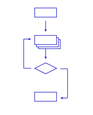
\includegraphics{images/repetition.png}
\end{center}
\end{block}
\end{column}

\begin{column}{0.5\textwidth}
\begin{block}{Selection}
\begin{center}
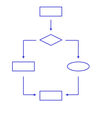
\includegraphics{images/selection.png}
\end{center}
\end{block}
\end{column}
\end{columns}
\end{frame}

\begin{frame}
\frametitle{Repetition}
\lstinputlisting{src/while.py}
\end{frame}

\begin{frame}
\frametitle{Repetition}
\lstinputlisting{src/while_1.py}
\end{frame}

\begin{frame}
\frametitle{Repetition}
\lstinputlisting{src/while_2.py}
\end{frame}

\begin{frame}
\frametitle{Selection}
\lstinputlisting{src/if_elif_else.py}
\end{frame}

\begin{frame}
\frametitle{A bit of boolean logic...}
\begin{table}
\begin{tabular}{lcl| l}
\texttt{not a} & & & returns True if \texttt{a} is False \\
\texttt{a and b} & {\tiny or} & \texttt{a \&\& b} & returns True if \texttt{a} \textbf{and} \texttt{b} are True \\
\texttt{a or b} & {\tiny or} & \texttt{a || b} & returns True if \texttt{a} \textbf{or} \texttt{b} is True \\
\hline
\texttt{a in b} & & & returns True if \texttt{a} is in \texttt{b} \\
\texttt{a not in b} & & & returns True if \texttt{a} is not in \texttt{b} \\
\end{tabular}
\end{table}

\begin{alertblock}{Question}
\begin{itemize}
\item Is \texttt{a and b or c} equivalent to \texttt{a and (b or c)}?
\end{itemize}
\end{alertblock}
\end{frame}

\begin{frame}
\frametitle{Exercises}
% FIXME
\begin{itemize}
\item \textbf{Q1} Give the range where the following statements are True:
\begin{itemize}
\item \texttt{a > 10 and a < 5}
\item \texttt{a > 10 or not a < 5}
\item \texttt{a < 10 or a > 5}
\item \texttt{a < 10 and a > 5}
\end{itemize}
\item \textbf{Q2} Print all even integers from 0 to 100.
\item \textbf{Q3} Write a small script that prints whether the product of two
variables \texttt{a} and \texttt{b} is negative, null or positive.
\item \textbf{Q4} Rewrite this without computing the product of those two
variables.
\end{itemize}
\end{frame}

\begin{frame}
\frametitle{Exercises}
\begin{itemize}
\item \textbf{Q5} Find the 100th element of the Fibonacci suite ($F_0 = 0$,
$F_1 = 1$, $F_{n + 1} = F_n + F_{n - 1}$)
\item \textbf{Q6}
Write a program that prints the numbers from 1 to 100. But for multiples of
three print "Fizz" instead of the number and for the multiples of five print
"Buzz". For numbers which are multiples of both three and five print
"FizzBuzz".
\end{itemize}
\end{frame}

\begin{frame}
\frametitle{Collection of objects}

A \textbf{list} is a \textbf{mutable} \textbf{ordered} collection of objects
that can be \textbf{indexed} or \textbf{sliced}.
\lstinputlisting{src/list.py}
\end{frame}

\begin{frame}
\frametitle{More on list}
\lstinputlisting{src/list_1.py}

\begin{alertblock}{Question}
\begin{itemize}
\item Can you find out what other methods can be used on a list? 
\end{itemize}
\end{alertblock}
\end{frame}

\begin{frame}
\frametitle{Looping over a list}
\lstinputlisting{src/for.py}
\end{frame}

\begin{frame}
\frametitle{Looping over a list}
\lstinputlisting{src/for_1.py}
\end{frame}

\begin{frame}
\frametitle{Looping over a list}
\lstinputlisting{src/for_2.py}
\end{frame}

\begin{frame}
\frametitle{Exercices}
\begin{itemize}
\item \textbf{Q1} Using a for loop, print all even integers from 0 to 100.
\item \textbf{Q2} Study the documention of the function \texttt{range}, and
rewrite the answer to the previous question without using \texttt{if}
\item \textbf{Q3} Modify your fibonacci script to keep track of all the members
of the suite.
\item \textbf{Q4} Write a script that ask the user for a number until the
answer is between 10 and 20. For each input, if the input is bigger than 20,
write a message that says "Smaller!". If the input is smaller than 10, write a
message that says "Bigger!"
\end{itemize}
\end{frame}

\begin{frame}
\frametitle{More on control flow}
\begin{itemize}
\item \texttt{\textbf{continue}}: allows to continue to the next iteration
\item \texttt{\textbf{pass}}: does nothing - used when a statement is required
syntatically
\item \texttt{\textbf{break}}: breaks out of the loop without continuing to the
next iteration
\end{itemize}

\lstinputlisting{src/loops.py}

\end{frame}

\begin{frame}
\frametitle{Other containers}
\begin{itemize}
\item A \textbf{tuple} is an \textbf{immutable} collection of objects. Once
created, you cannot change it.
\lstinputlisting{src/tuple.py}
\end{itemize}

\begin{alertblock}{Question}
\begin{itemize}
\item Why are tuples interesting?
\end{itemize}
\end{alertblock}
\end{frame}

\begin{frame}
\frametitle{Other containers}
\begin{itemize}
\item A \textbf{set} is a \textbf{mutable unordered} collection of unique objects.
\lstinputlisting{src/set.py}
\end{itemize}
\end{frame}

\begin{frame}
\frametitle{Other containers}
\begin{itemize}
\item A \textbf{dict} is a \textbf{mutable ordered} collection of pairs of keys
and values.
\lstinputlisting{src/dict.py}
\end{itemize}

\begin{alertblock}{Question}
\begin{itemize}
\item Do you think values should be unique?
\item Do you think keys should be unique?
\end{itemize}
\end{alertblock}
\end{frame}

\begin{frame}
\frametitle{Summary}
\begin{block}{Control Flow}
\begin{itemize}
\item While loop
\item For loop
\item If, elif, else
\end{itemize}
\end{block}

\begin{block}{Containers}
\begin{itemize}
\item \texttt{List}: \textbf{ordered, mutable} container
\item \texttt{Tuple}: \textbf{ordered, immutable} container
\item \texttt{Set}: \textbf{unordered, mutable} container of unique object
\item \texttt{Dict}: \textbf{unordered, mutable} container of pairs of keys and values.
\end{itemize}
\end{block}
\end{frame}

\begin{frame}
\frametitle{Exercises}
% FIXME
\begin{itemize}
\item \textbf{Q1} Given a list \texttt{l} of elements, how can you create a
sorted container of unique objects?
\item \textbf{Q2} The file \texttt{exo\_02.py} contains a dict. Ask to the
user for a key, and print the corresponding value. If the key doesn't exist,
print a nice error message.
\end{itemize}
\end{frame}


\begin{frame}
\frametitle{Manipulating files}
Two action can be done on files
\begin{itemize}
\item \textbf{Reading}
\lstinputlisting{src/reading.py}
\item \textbf{Writing}
\lstinputlisting{src/writing.py}
\end{itemize}
\end{frame}

\begin{frame}
\frametitle{More on reading files}
\lstinputlisting{src/reading_1.py}
\end{frame}

\begin{frame}
\frametitle{Exercises}
\begin{itemize}
\item \textbf{Q1} Write a script that computes the number of letter \textbf{i}
in the first sentence.
\item \textbf{Q2} Write a script that prints the first and last letter of each
line.
\item \textbf{Q3} Write a script that prints all the capital letters of the
text.
\end{itemize}
\end{frame}

\begin{frame}
\frametitle{Writing functions}
\lstinputlisting{src/function.py}
\end{frame}

\begin{frame}
\frametitle{Arguments...}
\textbf{Arguments} can be of two types:
\begin{itemize}
\item \textbf{Mandatory} arguments
\item \textbf{Optional "keyword"} arguments
\end{itemize}

\lstinputlisting{src/function_1.py}
\end{frame}

\begin{frame}
\frametitle{Exercises}
\begin{itemize}

\item \textbf{Q1} Write a function \texttt{ceil} that returns the smallest
integral value superior or equal to the input. Tip: cast the input to an
integer using \texttt{int(x)}.
\item \textbf{Q2} Write a function \texttt{floor} that returns the smallest
integral value superior or equal to the input
\item \textbf{Q3} Write a function \texttt{round} that takes in input a
number \texttt{a}, and returns the closest integer.
\item \textbf{Q4} Write a Fibonacci function that returns the Fibonacci
elements up to an argument \texttt{n}.
\item \textbf{Q5} In a file called \texttt{ngs.py} write a function
\texttt{gc\_content} that takes as argument a string, and outputs the
gc\_content.
\item \textbf{Q6} Use this function to compute the gc content for each line of
the file \texttt{dna\_sequence.txt}
\end{itemize}
\end{frame}

\section{Standard libraries and modules}
\begin{frame}
\frametitle{All batteries included...}
\begin{center}
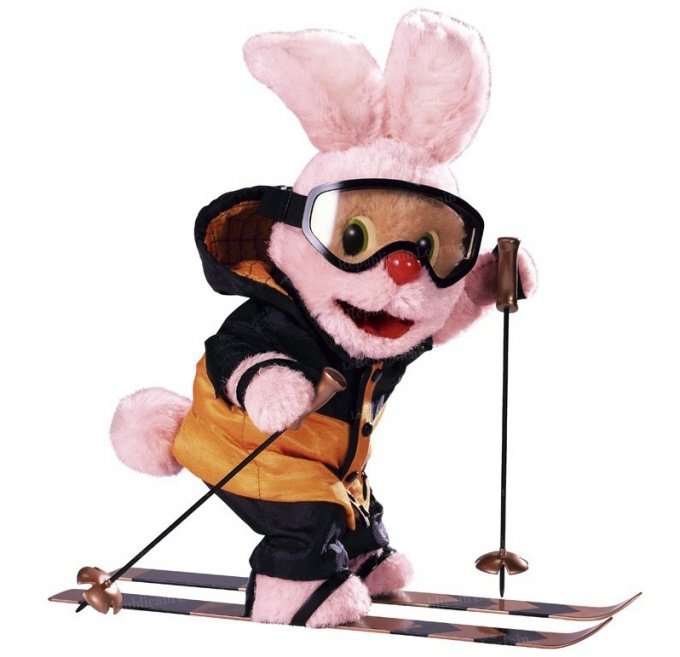
\includegraphics{images/un-lapin-tout-terrain-duracell.jpg}
\end{center}
\end{frame}

\begin{frame}
\frametitle{Modules}
\begin{block}{Modules}
\textbf{modules} are file containing Python code.
\end{block}

\vspace{1em}
Consider a module \texttt{fibonacci.py} containing the function \texttt{fibo}
\lstinputlisting{src/modules.py}
\lstinputlisting{src/modules_1.py}
\end{frame}

\begin{frame}
\frametitle{Executing modules as scripts}
\begin{block}{Using}
\texttt{python module.py}
\end{block}

\vspace{1em}

This will execute the module as if you import it, but its name will not be
the same:

\lstinputlisting{src/modules_2.py}

That means you can protect some of the code from being run when the module is
imported

\end{frame}

\begin{frame}
\frametitle{Example}
\lstinputlisting{src/script_vs_module.py}
\vspace{2em}
The second part of the script will not be executed when importing the module.

\begin{alertblock}{Question}
\begin{itemize}
\item Why do you think I named the function \texttt{print\_} ?
\end{itemize}
\end{alertblock}

\end{frame}

\begin{frame}
\frametitle{The standard library}
\end{frame}

\begin{frame}
\frametitle{maths}
\begin{tabular}{llllll}
acos & acosh & asin & asinh & atan & atan2\\
atanh & ceil & copysign & cos & cosh & degrees \\
e & erf & erfc & exp & expm1 & fabs \\
factorial & floor & fmod & frexp & fsum & gamma \\
hypot & isinf & isnan & ldexp & lgamma & log \\
log10 & log1p & modf & pi & pow & radians \\
sin & sinh & sqrt & tan & tanh & trunc \\
\end{tabular}

\end{frame}

\begin{frame}
\frametitle{os}
Everything that is linked to the os.
\begin{block}{Manipulating paths}
\begin{tabular}{lll}
os.path.abspath(".") & & /home/nelle/Projects \\
os.path.join("a", "b") & & a/b \\
os.path.split("a/b") & & ["a", "b"] \\
os.path.exists(path) & & True or False \\
os.path.isfile(path) & & True or False \\
os.path.isdir(path) & & True or False \\
os.path.basename('presentation/slides.pdf') & & slides.pdf \\
os.path.dirname("presentation/slides.pdb") & & presentation \\
\end{tabular}
\end{block}

\end{frame}
\begin{frame}
\frametitle{Example}
\lstinputlisting{src/os_.py}
\end{frame}

\begin{frame}
\frametitle{glob}
\begin{block}{Filename globbing utility.}
\lstinputlisting{src/glob_.py}
\end{block}
\end{frame}

\begin{frame}
\frametitle{shutil}

\begin{block}{Utility functions for copying and archiving files and directory
trees.}
\begin{tabular}{lll}
shutil.copy & & \\
shutil.copytree & & \\
shutil.rmtree & & \\
shutil.make\_archive & & \\
\end{tabular}
\end{block}
\end{frame}

\begin{frame}
\frametitle{Exercises}
\end{frame}

\begin{frame}
\frametitle{Debugging - the pdb module}
\begin{block}{Python Debugger}
\lstinputlisting{src/pdb_.py}
\end{block}
\end{frame}

\end{document}
